\documentclass{article}
\usepackage{color,graphicx}
\usepackage{natbib}
\bibliographystyle{plainnat}
\usepackage[utf8]{inputenc}
\usepackage[swedish]{babel}


\author{Henrik Andersson}
\title{Probabilistisk våghöjdsprognos}

\begin{document}
\maketitle
    
\begin{abstract}
Våghöjd, risk \ldots
\end{abstract}

\section{Introdukton}

\citep{deo01}

\section{Metod}

\subsection{Data}

Observationer av våghöjd, riktning och period ~(Fig.~\ref{fig:data-test}) från SMHIs arkiv av öppna data från \citet{smhi}.

\begin{figure}
    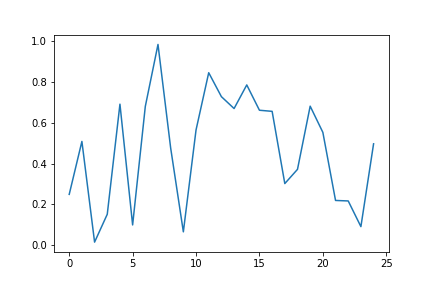
\includegraphics{fig/test}
    \caption{Test figur}
    \label{fig:data-test}
\end{figure}

\section{Resultat}

\section{Diskussion}


\bibliography{waves}




\end{document}